\begin{center}
  \scalebox{1.0}{
    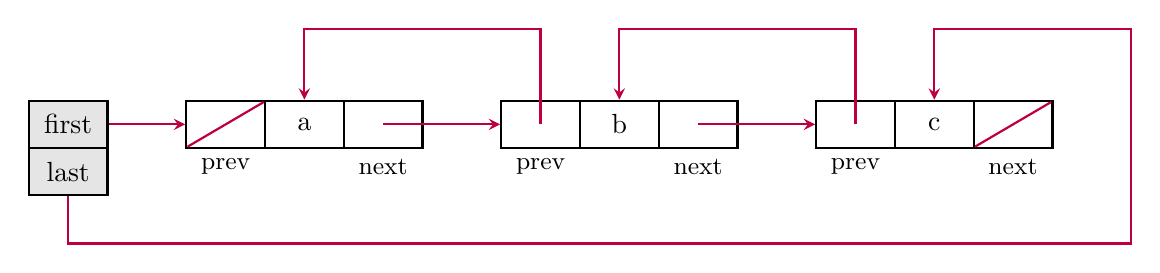
\begin{tikzpicture}[]
      \coordinate (origo) at (0mm,-6cm);
      
      \tikzstyle{cell} = [
        rectangle,
        draw=black,
        thick,
        anchor=west,
        minimum width=10mm,
        minimum height=6mm,
      ]
      \tikzstyle{celllabel} = [
        draw=none,
        anchor=north,
        align=center
      ]
      
      \tikzstyle{arrow} = [thick,->,>=stealth, draw=purple]
      
      % object
      \node[cell,fill=black!10] (cellFirst) at ([xshift=0mm] origo) {first};
      \node[cell,fill=black!10] (cellLast) at ([xshift=0mm,yshift=-6mm] origo) {last};
      
      % link 1
      \node[cell] (cell1prev) at ([xshift=20mm] origo) {};
      \node[cell] (cell1data) at ([xshift=30mm] origo) {a};
      \node[cell] (cell1next) at ([xshift=40mm] origo) {};A
      \node[celllabel] (cell1prevLabel) at ([xshift=0mm] cell1prev.south) {\small prev};
      \node[celllabel] (cell1nextLabel) at ([xshift=0mm] cell1next.south) {\small next};
      
      % link 2
      \node[cell] (cell2prev) at ([xshift=60mm] origo) {};
      \node[cell] (cell2data) at ([xshift=70mm] origo) {b};
      \node[cell] (cell2next) at ([xshift=80mm] origo) {};
      \node[celllabel] (cell2prevLabel) at ([xshift=0mm] cell2prev.south) {\small prev};
      \node[celllabel] (cell2nextLabel) at ([xshift=0mm] cell2next.south) {\small next};
      
      % link 1
      \node[cell] (cell3prev) at ([xshift=100mm] origo) {};
      \node[cell] (cell3data) at ([xshift=110mm] origo) {c};
      \node[cell] (cell3next) at ([xshift=120mm] origo) {};
      \node[celllabel] (cell3prevLabel) at ([xshift=0mm] cell3prev.south) {\small prev};
      \node[celllabel] (cell3nextLabel) at ([xshift=0mm] cell3next.south) {\small next};
      
      % forward
      \draw[arrow] (cellFirst.east) -- (cell1prev.west);
      \draw[arrow] (cell1next.center) -- (cell2prev.west);
      \draw[arrow] (cell2next.center) -- (cell3prev.west);
      
      % backward
      \draw[arrow] (cellLast.south) |- ([yshift=-6mm] cellLast.south) -| ([yshift=9mm,xshift=25mm] cell3data.north) -| (cell3data.north);
      \draw[arrow] (cell3prev.center) |- ([yshift=9mm] cell2data.north) -| (cell2data.north);
      \draw[arrow] (cell2prev.center) |- ([yshift=9mm] cell1data.north) -| (cell1data.north);
      \draw[overlay,thick,draw=purple] ([xshift=-0.3mm,yshift=-0.3mm] cell1prev.north east) -- ([xshift=0.3mm,yshift=0.3mm] cell1prev.south west);
      \draw[overlay,thick,draw=purple] ([xshift=-0.3mm,yshift=-0.3mm] cell3next.north east) -- ([xshift=0.3mm,yshift=0.3mm] cell3next.south west);
    \end{tikzpicture}
  }
\end{center}
